\documentclass[times,twoside]{zHenriquesLab-StyleBioRxiv}
\renewcommand{\familydefault}{\sfdefault}
\usepackage{wrapfig} % Allows in-line images
\usepackage[round]{natbib}
\setcitestyle{numbers,open={ (},close={)}}
% \usepackage[superscript]{cite}
\usepackage{blindtext}
\usepackage{color}
\usepackage{xcolor}
\usepackage{multicol}
\usepackage{float}
\usepackage[colorinlistoftodos]{todonotes}
\floatplacement{figure}{H}
\usepackage{url,multirow,morefloats,floatflt,cancel,tfrupee}
%=== quotation
\usepackage{csquotes}
%=== inline lists
\usepackage{paralist}
%=== Tables
\usepackage{booktabs}


\renewcommand \thesection{\arabic{section}}
\renewcommand \thesubsection{\arabic{section}.\arabic{subsection}}


%===== COMMENTS \& NOTES =============
\usepackage[margin=true,inline=false,index=true]{fixme}
\fxsetup{
    status=draft,
    layout=inline,
    theme=colorsig,
    targetlayout=colorcb,
    mode=multiuser
}
%-- fixme author registration
\FXRegisterAuthor{da}{eda}{DA}
\FXRegisterAuthor{db}{edb}{DB}% etc

%=== TIKZ graphics
\usepackage{tikz}
\usetikzlibrary{automata,positioning,shapes.geometric}
\usepackage{cleveref}


%=== COMMAND DEFINITIONS
\def \figPath{figs/}

%=== DOCUMENT SETTINGS
\onecolumn
\leadauthor{XXX} 

\begin{document}

%===== BEGIN DOCUMENT=================
\title{GBM communities exploiting the interactions between ploidy and host physiology}
\author{ First A. Author, Second B. Author, and Third C. Author }



\maketitle


\section*{INTRODUCTION}
GBM remains uniformly lethal, with a median survival of 14-16 months and a 5-year survival rate of less than 3\%, despite aggressive therapy consisting of surgery, radiation, and chemotherapy. Aging is a main risk factor for GBM, however to date how the aging process affects GBM remains unknown. Strikingly, in people aged 65 and above, GBMs prognosis is even more dismal, with overall survival of less than 7 months upon diagnosis, suggesting that the aging process has a direct role in GBM aggressiveness. Polyploidy (elevated genomic content) is a hallmark of cancer thought to play a role in cancer progression and to facilitate rapid tumor evolution to survive anti-cancer therapies. However, while polyploidy confers significant advantages to cancer cells, it comes at the expense of higher metabolic demand to meet the requirements to synthesize higher amounts of DNA, RNA and proteins. While the exact metabolic requirements of polyploidy remain largely unknown, our preliminary data suggests that the availability of metabolic substrates in the environment (e.g. glucose, phosphate, oxygen) drives different cell fate decisions (e.g. proliferate, migrate or die) in cancer cells of different ploidy. This puts forward the idea that the metabolic state of the patient is crucial in shaping the evolution of tumors and in allowing for polyploid cancer cells to thrive. Interestingly, polyploidy has been recently shown to increase in the brain with age, supporting the idea that aging drives an environment in the brain conducive to high ploidy cancer cells to thrive. Our central hypothesis is that a major determinant of the variable GBM cell fate in response to the metabolic state of the host is determined by intra-tumoral differences in ploidy. This hypothesis has three implications: (1) that the age-driven changes in global and local metabolic conditions tip the balance of the GBM community favoring GBM cells of variable ploidy; (2) that adaptive therapeutic strategies designed to metabolically “rejuvenate” the host environment have the potential to restructure the GBM cellular communities. We will address our hypothesis with the following three specific aims:

Aim 1: Identify how ploidy of GBM cells modulates thresholds for cell state transition with respect to resource availability. Infiltration is the first response of cells to hypoxia and recent evidence suggests that infiltration is an early phenotype in the evolution of GBM. We will genetically engineer 5 GBM cell lines to obtain 2N and 4N lineages for each. Using these as a model, we will test how exposure to variable gradients of glucose, hypoxia and phosphate affect their migratory patterns. This data will be used to calibrate a partial differential equation (PDE) model to recapitulate how each lineage migrates in response to reduced resource availability. The inferred lineage specific diffusion coefficients will be analyzed with respect to the ploidy of each lineage to verify the expectation that high ploidy cells migrate more rapidly in response to resource limitations.

Aim 2: Model how changes in GBM cell ploidy composition and phenotype affect GBM and inform a personalized adaptive radiation regimen. We will extend our stochastic state space model of the brain (S3MB)
to the 3D setting. We will apply this model to a retrospective cohort of 5 primary GBM patients and will use BOLD imaging to quantify the spatial distribution of oxygen in tumors prior to surgery. Geo-tagged surgical specimens collected at the time of surgery will be sequenced and T1-weighted scans will inform the coordinates of the resection cavity and of enhancing regions around the resection cavity. This data will be integrated will serve as initial conditions to SSMB. The model will simulate regrowth of the enhancing region into a recurrent tumor. The temporal and spatial dynamics of recurrence will be compared to those measured on follow-up scans of the same patient. This will allow us to calibrate the model and to verify whether assumptions on the relation between ploidy, resource availability and cell fate generalize from the in-vitro to the in-vivo setting. The calibrated model will be validated on 5 additional patient-matched primary and recurrent GBM. Once calibrated, SSMB will be used as a hypothesis generating model to evaluate the potential of administering a spatially heterogeneous SBRT regimen targeting low-resource tumor regions with higher radiation dose to delay recurrence.

Aim 3: Evaluate how age and metabolic “rejuvenation” strategies affect the ploidy composition and growth of the GBM. Based on published evidence demonstrating that aging promotes an increase in glucose levels as well as changes in stiffness and oxygenation in the brain, we hypothesize that aging drives poor prognosis in GBM by providing the optimal environment for GBM cells. In this aim, we will use the model developed in Aim 2 to generate predictions to guide pre-clinical research using young and old mice as models to test if and how aging contributes to the ploidy evolution in GBM. Moreover, informed by this mathematical model we will test if modulating host physiology with FDA-approved drugs that have been shown to metabolically “rejuvenate” the host (e.g. anti-diabetic drugs, osteoporosis medications, phosphate and oxygen modulating drugs) can modulate ploidy evolution and thereby sensitize older GBM patients to standard of care therapies.

Impact.   Together we expect these aims to contribute to a better understanding of how microenvironment resources shape the community of GBM cells of varied ploidy and how to best modulate host physiology to delay recurrence and progression.

\section{METHODS}

\subsection{Statistical analysis} 
Aneuploidy score, genome doublings: 10.1016/j.ccell.2018.03.007

Gene expression data - mRNA expression z-scores relative to diploid samples (RNA Seq V2 RSEM): cbioportal, accessed on 02.11.2022

Oxygenation status of organs/tissues: PMID: 32786046, 30899601

Where ranges were provided (e.g.: kidney cortex 45-50), mean value was selected from given range (e.g. 47.5). Where possible, reference was taken from PMID: 32786046 as a resource with more normal tissues; PMID: 30899601 was selected if the tissue was missing or less precise in the first source

\subsection{ODE model} 

\subsection{Stochastic State-Space Model} 

\section{RESULTS}
\subsection{Ploidy, Oxygen and Glucose in aged and young environments}

\begin{figure}
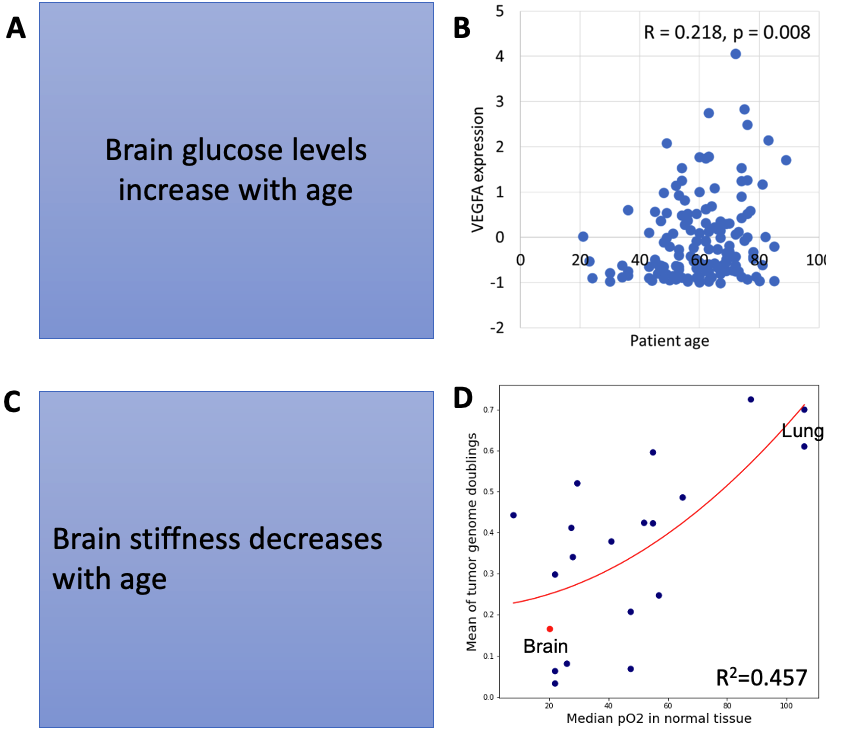
\includegraphics[width=0.5\textwidth]{figs/Fig1.png}
\caption{\textbf{Age associated molecular, metabolic and functional changes.}
A) XX.
B) XX.
C) XX.
D) XX.
} 
\label{fig:stats}
\end{figure}

\subsection{ODE model of Glucose dependent migration} 

\subsection{Stochastic State-Space Model of the Brain} 

\section*{DISCUSSION}

\section*{SUPPLEMENTARY INFORMATION}

\section*{REFERENCES}

\bibliography{references}
\bibliographystyle{unsrt}


\end{document}
